\chapter{Embedded Software Concepts}
\label{chap:SensorConcepts}
%In this chapter, I will cover in detail the code and DSP techniques used in the data flow of the sensor designs covering both the analog front end for the real sensors and the software DSP and data fusion techniques for the synthetic sensors.
Any embedded design is a combination of both hardware and firmware. The WHIP is no different. The firmware was developed to allow for future expansion and should serve as a starting point, not an end point for development. All firmware was written in the C language. The development environment was Atmel Studio V6.2\cite{AtmelStudio}. The following sections cover the code generated for this firmware in the following groups. First the low level driver for the ECG and \spo2 chips; then the integration with the Atmel Software Framework and, finally, the driver code state machine

\begin{figure}
	\begin{center}
		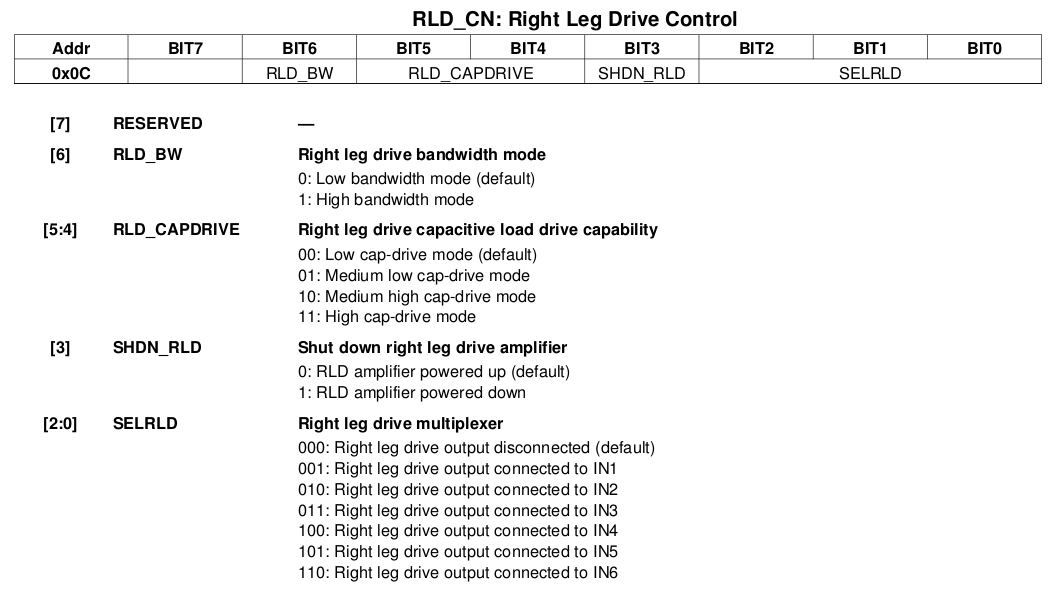
\includegraphics[scale=1,width=0.9\textwidth]{Images/ADS1293_RLD_CN_modified.png} 
		\caption{Excerpt from ADS1293 Data Sheet Describing the RLD CN Register}
		\label{fig:ADS1293_RLD_CN}
	\end{center}
\end{figure}

\section{Chip Driver Firmware}

Both the AFE4490 \spo2 IC and the ADS1293 ECG IC offered attractive features settable in software, including gain amplifiers and sample rate. However, these features, while flexible, required a substantial investment in understanding the configuration registers present in both chips. An intermediate C\# program was written to ingest specifications from the data sheet and produce a header file with descriptive \#define statements that could be used to create self-documenting code. Consider \Cref{fig:ADS1293_RLD_CN}, as an example, an excerpt from the ADS1293 data sheet shows a  bit-mapped register, responsible for several functions related to the right leg drive circuitry(RLD) of the ADS1293. The code in \cref{fig:ADS1293_Defines} was generated to simplify code generation and increase readability. The use of masking and bit shifting ensures that invalid bits do not unintentionally have side effects; and the descriptive bit names help document the code to communicate meaning. Examining the ADS1293 initialization routine in \Cref{fig:ADS1293_INIT} shows how effective this strategy can be. The use of a well organized array allows for all settings to be seen at a glance. This approach does not eliminate the need for the data sheet while programming, but by using define statements to create readable alternatives to hard coded binary numbers we greatly increase the maintainability of the code base. Both ICs received a similar treatment and a library of basic functionality was written for each chip.

\begin{figure}
	\begin{center}
\begin{lstlisting}[frame=single]
//RLD_CN
#define ADS1293_RLD_CN  0x0C

#define RLD_BW _BV(6)
#define RLD_CAPDRIVE(n) (((n)&3)<<4)
#define RLD_LOW_DRIVE 0
#define RLD_MED_LOW_DRIVE 1
#define RLD_MED_HIGH_DRIVE 2
#define RLD_HIGH_DRIVE 3
#define SHDN_RLD _BV(3)
#define SELRLD(n) (((n)&7)<<0)
\end{lstlisting}
		\caption{Self Documenting Define Statements for ADS1293 ``ADS1293.h''}
		\label{fig:ADS1293_Defines}
	\end{center}
\end{figure}


\begin{figure}
	\begin{center}
\begin{lstlisting}[frame=single,morekeywords={ECG_INIT_DATA}]
ECG_INIT_DATA ads1293Defaults[] = {
{ADS1293_FLEX_CH1_CN, POS(IN4)|NEG(IN5)}, 
{ADS1293_CMDET_EN,    CMDET(IN4)|CMDET(IN5)},
{ADS1293_CMDET_CN,    CMDET_BW | CMDET_HIGH_DRIVE},
{ADS1293_RLD_CN,      SELRLD(IN6)},
{ADS1293_AFE_SHDN_CN, SHDN_SDM(2)|SHDN_SDM(3)|
                      SHDN_INA(2)|SHDN_INA(3)},
{ADS1293_R2_RATE,     R2_RATE_4},
{ADS1293_R3_RATE_CH1, R3_RATE_8},
{ADS1293_R1_RATE,     R1_DOUBLE_CH1},
{ADS1293_DRDYB_SRC,   DRDYB_SRC_CH1ECG},
{ADS1293_MASK_DRDYB,  DRDYB_MASK_NONE},
{ADS1293_CH_CNFG,     E1_EN},
{ADS1293_OSC_CN,      STRTCLK|EN_CLKOUT},
{ADS1293_CONFIG,      START_CON}
};

void ECG_begin()
{
  for (int i=0;
       i<sizeof(ads1293Defaults)
         /sizeof(ads1293Defaults[0]);
         i++)
  {
    ECGsingleWrite(ads1293Defaults[i].address,
                   ads1293Defaults[i].data);
  }
}
\end{lstlisting}
		\caption{Initialization Code for ADS1293 ``ADS1293.c''}
		\label{fig:ADS1293_INIT}
	\end{center}
\end{figure}



\section{Atmel Software Framework (ASF)}
The Atmel website clearly sums up the ASF:

\begin{quotation}
The Atmel Software framework is a MCU software library providing a large collection of embedded software for Atmel flash MCUs: megaAVR, AVR XMEGA, AVR UC3 and SAM devices.

It  simplifies the usage of microcontrollers, providing an abstraction to the hardware and high-value middlewares
ASF is designed to be used for evaluation, prototyping, design and production phases
ASF is integrated in the Atmel Studio IDE with a graphical user interface or available as standalone for GCC, IAR compilers
ASF can be downloaded for free. \cite{AtmelStudio}
\end{quotation} 
% http://www.atmel.com/tools/avrsoftwareframework.aspx)

The two primary benefits to this project, provided by the ASF are its abstraction layer across different hardware devices, and its collection of embedded libraries.

Over the course of development several processors were used. All devices were manufactured by Atmel, but spanned different chip families. Early development used the megaAVR series of 8 bit processors, while the final design used the 32 bit UC3 series. The details of accessing the low level configuration registers of any specific hardware were ``hidden'' from the functional code by utilizing the ASF. The word ``hidden'' is in quotes because, often the low level code had to be rewritten by the programmer. But, this was well worth the time invested to keep the higher level libraries unchanged. Specifically, the SD card/FAT libraries allowed for a POSIX file interface to simplify sample storage, and the USB libraries made interfacing to a computer trivial; allowing the programmer to focus on interfacing with the relevant sensors and not on timing details of the USB specification.

\section{Main State Machine}

The basic state machine of the WHIP firmware, shown in \cref{fig:flowchart_main}, was simplistic, but robust. Data was pipelined directly from both ECG and \spo2 devices to a double buffered memory location By making use of the DMA channels on the micro controller . Then, another DMA channel wrote the collected data to the SD card. The CPU only intervened once the write-buffer was filled, at which point the buffers were swapped. The only other mode the device can enter is USB mode. Upon connection to USB power data collection is halted and all files are flushed and closed in preparation for download. When USB power is removed, data collection starts again. 

\begin{figure}
	\begin{center}
		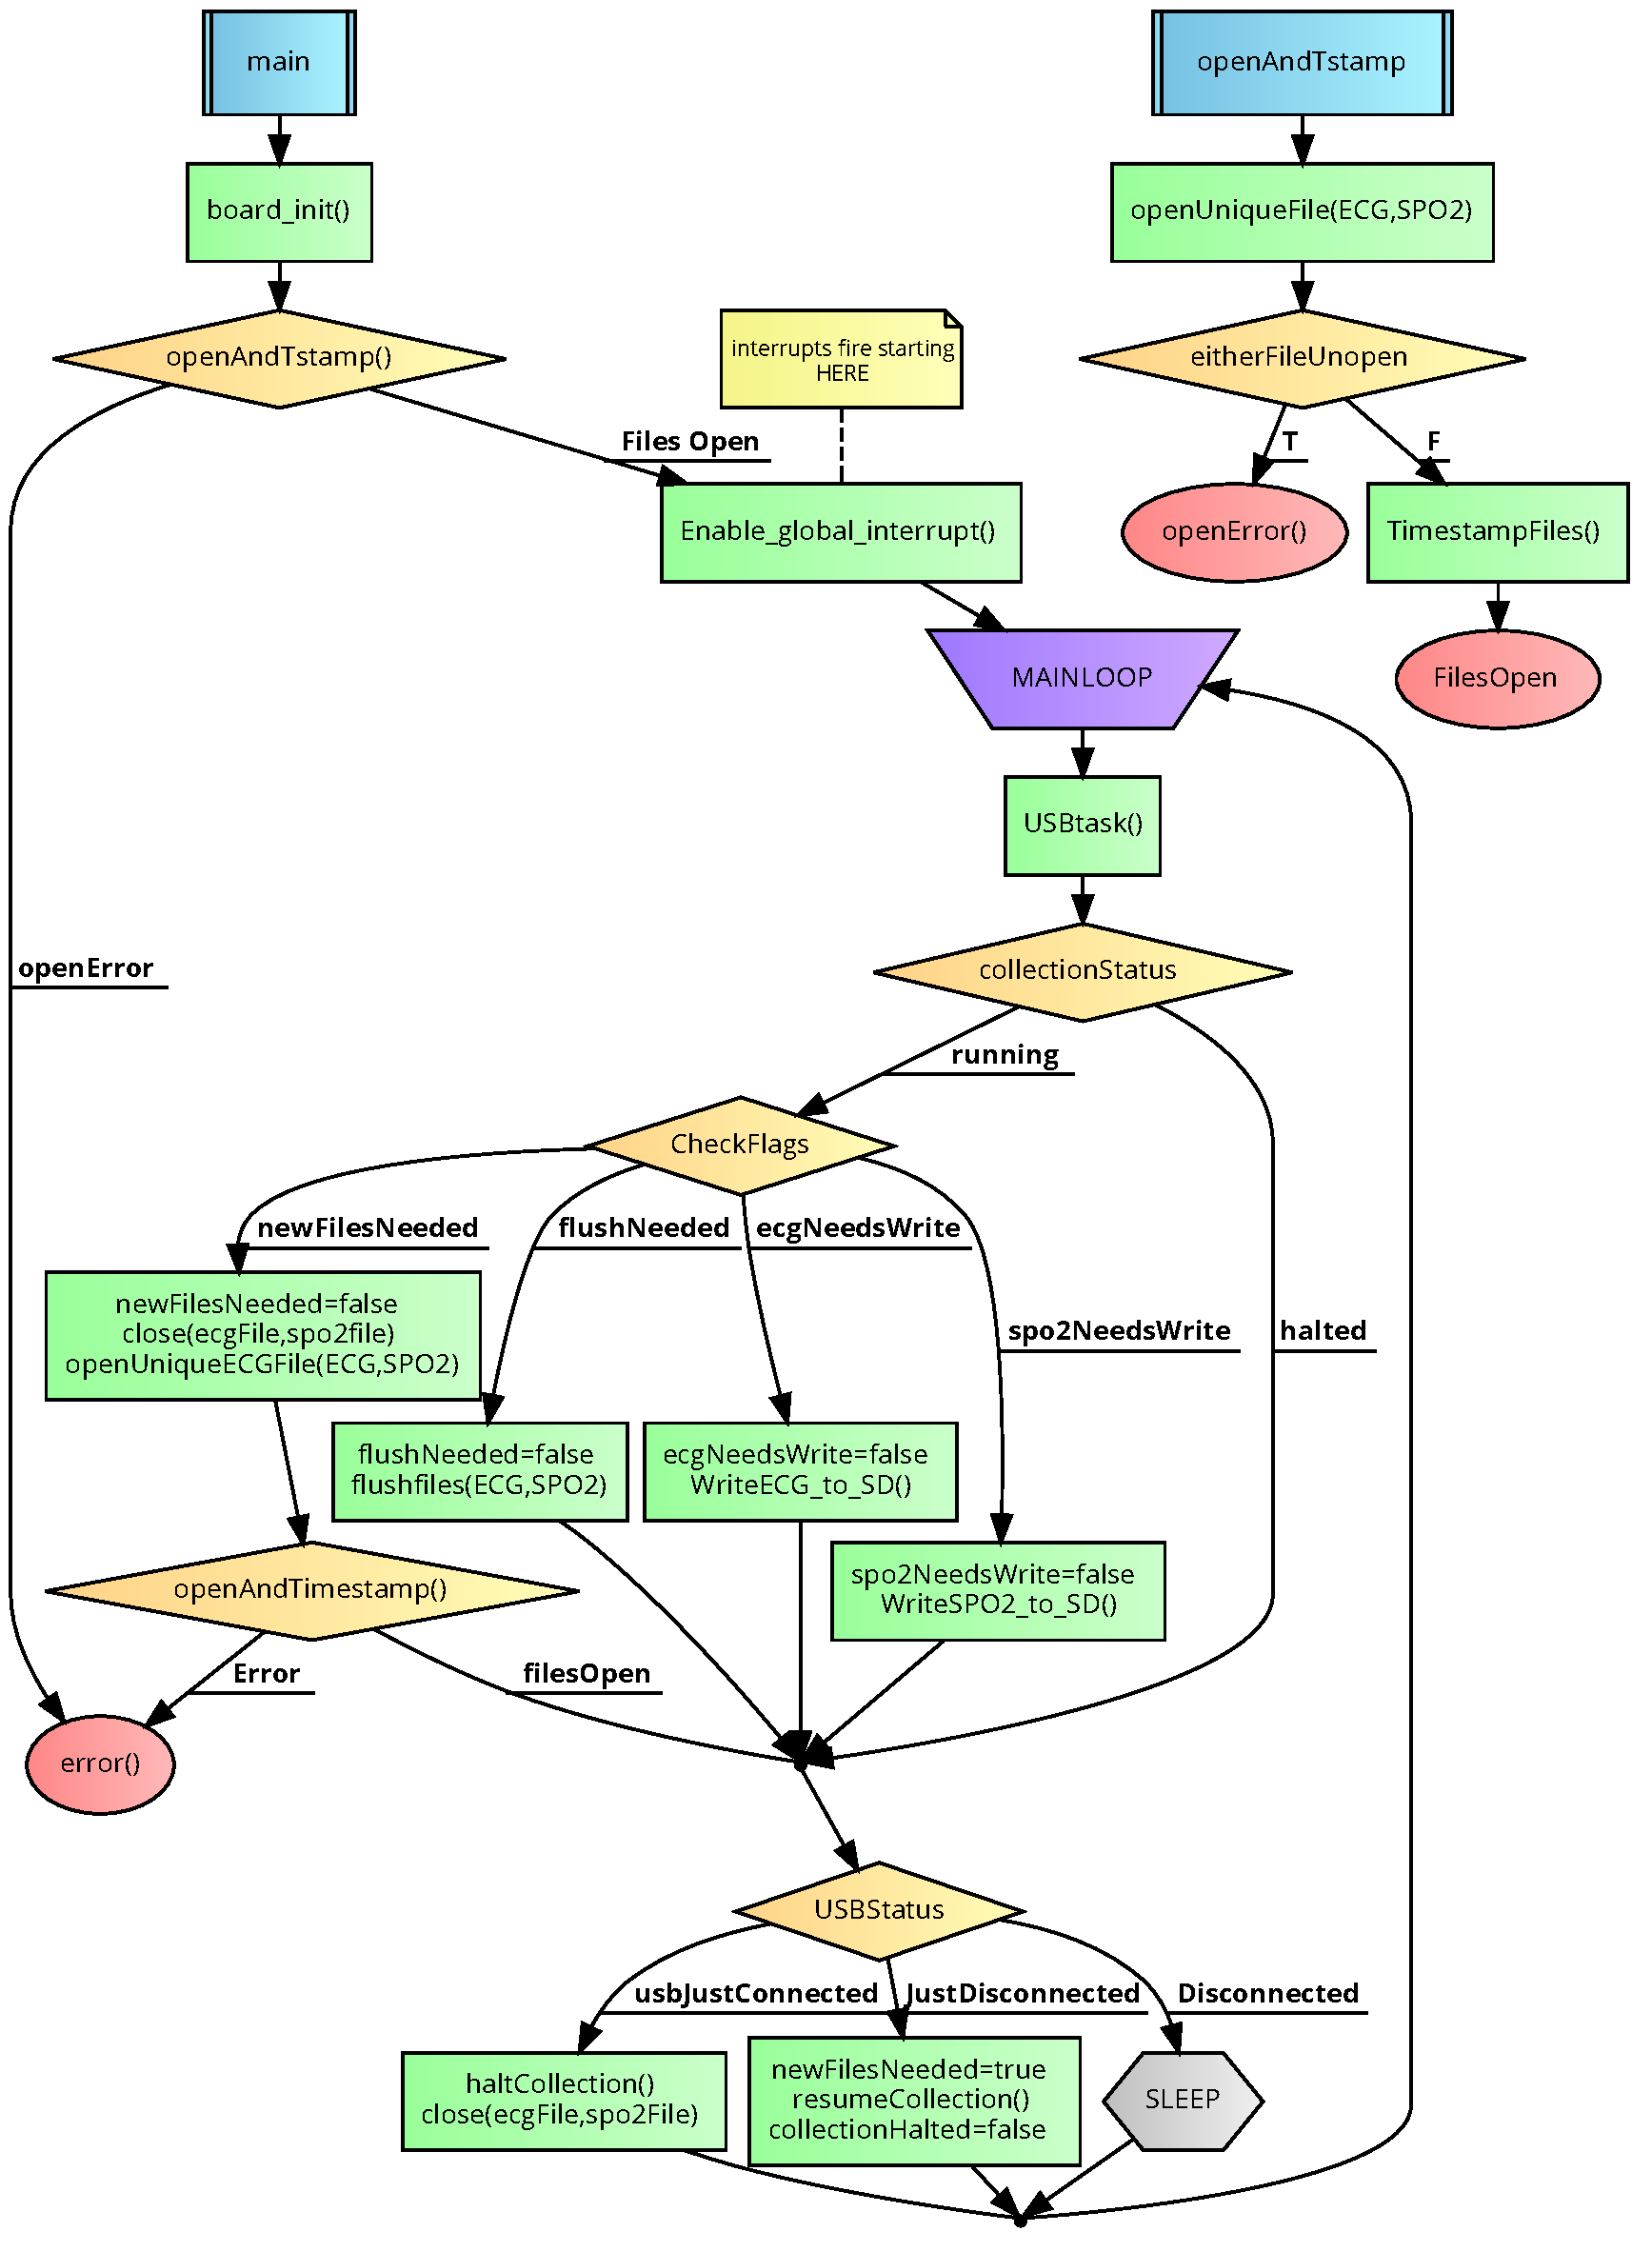
\includegraphics[scale=1,width=0.9\textwidth]{Images/FlowChartMain.pdf} 
		\caption{Main Function, Functional Flowchart}
		\label{fig:flowchart_main}
	\end{center}
\end{figure}

\section {Interrupt Service Routines (ISRs)}
Microcontrollers best utilize resources when not polling, using busy loops, waiting for events to occur. Interrupt Service Routines (ISRs) allow for low level tasks to be interrupted in favor of higher priority tasks. The ATUC3 line of microcontrollers offers many Interrupt sources. The two most important, from a WHIP firmware standpoint, are the Data Received interrupts for the AFE4490 \spo2 and the ADS1293 ECG chips. \cref{fig:flowchart_ISR} shows that both interrupts are similar. Both buffer incoming data until the buffer is full. When a buffer is full, a new buffer is swapped into place and the old buffer can be sent to the SD card for storage. The \spo2 interrupt contains one extra feature; a dynamic brightness calibration to prevent saturation of the pleth sensor. Other differences in the \spo2 ISR are not additional features just a reflection of the data delivered by the pleth sensor, two channels of data, and an additional two channels of intensity data.
\begin{figure}
	\begin{center}
		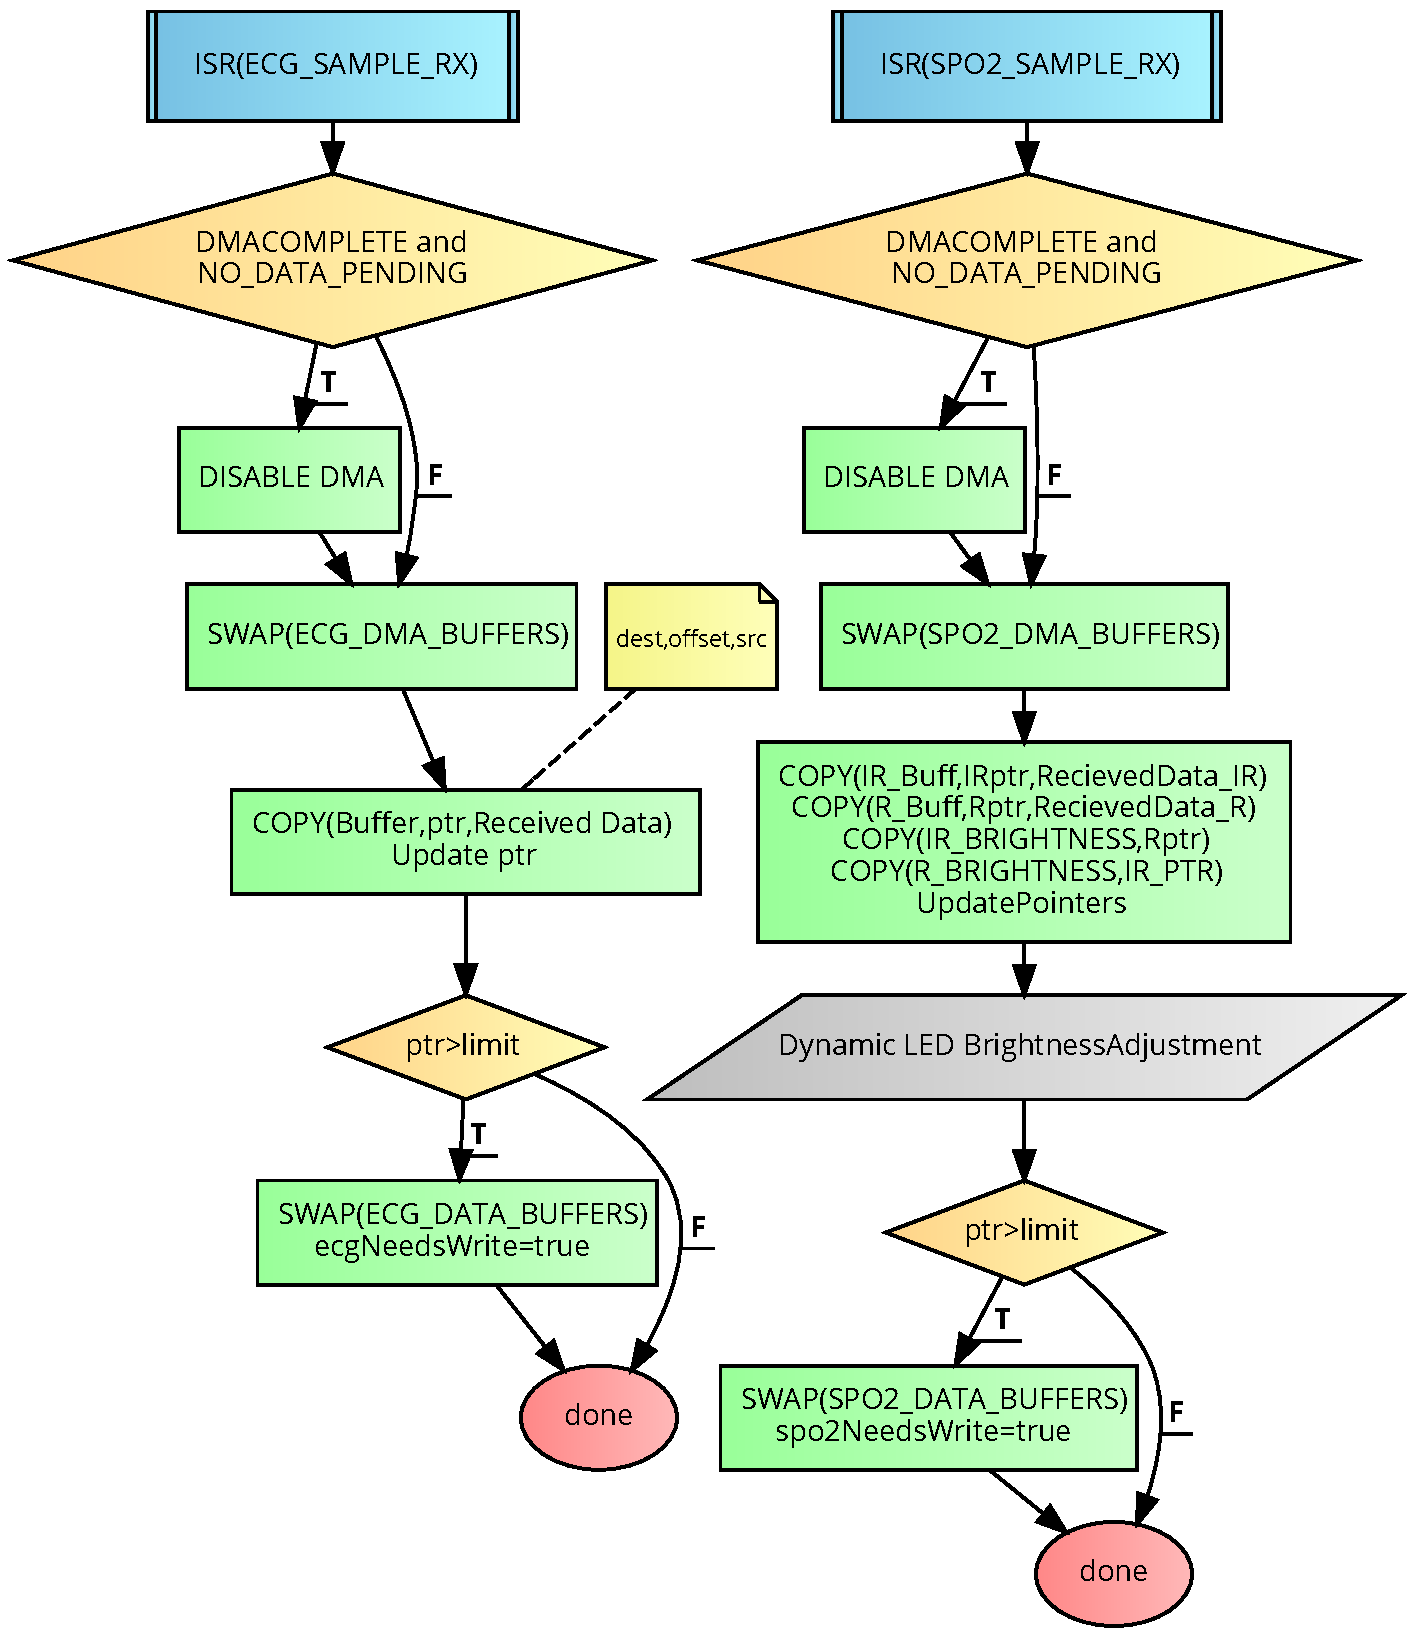
\includegraphics[scale=1,width=0.9\textwidth]{Images/FlowChartISR.pdf} 
		\caption{ISR Functional Flowchart}
		\label{fig:flowchart_ISR}
	\end{center}
\end{figure}

